\section{Data Generation}

\begin{frame}{Training Dataset: Features}

    The dataset consists of $n = 10^4$ observations with 3 features and 1 target variable.\\\vspace{0.3cm}
    \pause\textbf{Features:}
    \begin{itemize}
        \item $ \boldsymbol{X}_{\text{train}} = (X_{\text{train}\,1}, X_{\text{train}\,2}, X_{\text{train}\,3}) \sim \mathcal{N}(\boldsymbol{\mu}_{\text{train}}, \boldsymbol{\Sigma}_{\text{train}}) $
        \item $ \mu_{\text{train}\,i} \sim \mathcal{U}_{[0,1]} $ for $ i = 1, 2, 3 $
        \item $ [\boldsymbol{\Sigma}_{\text{train}}]_{i,j} \sim \mathcal{U}_{[-1,1]} $ for $ i, j = 1, 2, 3 $
    \end{itemize}
    \vspace{0.3cm}
    \textbf{\underline{Note}:} The $\boldsymbol{\Sigma}$ randomly generated has been transformed to a symmetric and positive semidefinite matrix by computing $\boldsymbol{\Sigma}\boldsymbol{\Sigma}^T$. 

\end{frame}

\begin{frame}{Training Dataset: Target Variable}
    Building the \textbf{target variable} $Y\in\{0,1\}$:

    \begin{enumerate}
        \item $$ 
        z = \beta_0 + \sum_{i=1}^3 \beta_i x_i + \sum_{i=1}^3 \beta_{ii} x_i^2 + \sum_{i=1}^{2} \sum_{j=i+1}^3 \beta_{ij} x_i x_j\,,   \quad \beta_{\cdot} \sim \mathcal{U}_{[-1,1]}
        $$
        \item $$ p = \frac{1}{1 + e^{-z}}$$
        \item $$ Y \sim \text{Be}(p)$$
    \end{enumerate}
\end{frame}

\begin{frame}{Testing Dataset}

    Same dataset structure as the train set, but:
    \begin{itemize}
        \item $ \boldsymbol{X}_{\text{shift}} = (X_{\text{shift}\,1}, X_{\text{shift}\,2}, X_{\text{shift}\,3}) \sim \mathcal{N}(\boldsymbol{\mu}_{\text{shift}}, \boldsymbol{\Sigma}_{\text{shift}}) $
        \item $ \boldsymbol{\mu}_{\text{shift}} = \mathcal{Q}_{0.05}(\boldsymbol{X}_{\text{train}})$
        \item $\boldsymbol{\Sigma}_{\text{shift}}$ generated in the same way as $\boldsymbol{\Sigma}_{\text{train}}$ (but $\boldsymbol{\Sigma}_{\text{shift}}\neq\boldsymbol{\Sigma}_{\text{train}}$)
    \end{itemize}
    
\end{frame}

\begin{frame}{Original and Shiftd Features}
    \begin{figure}
        \centering
        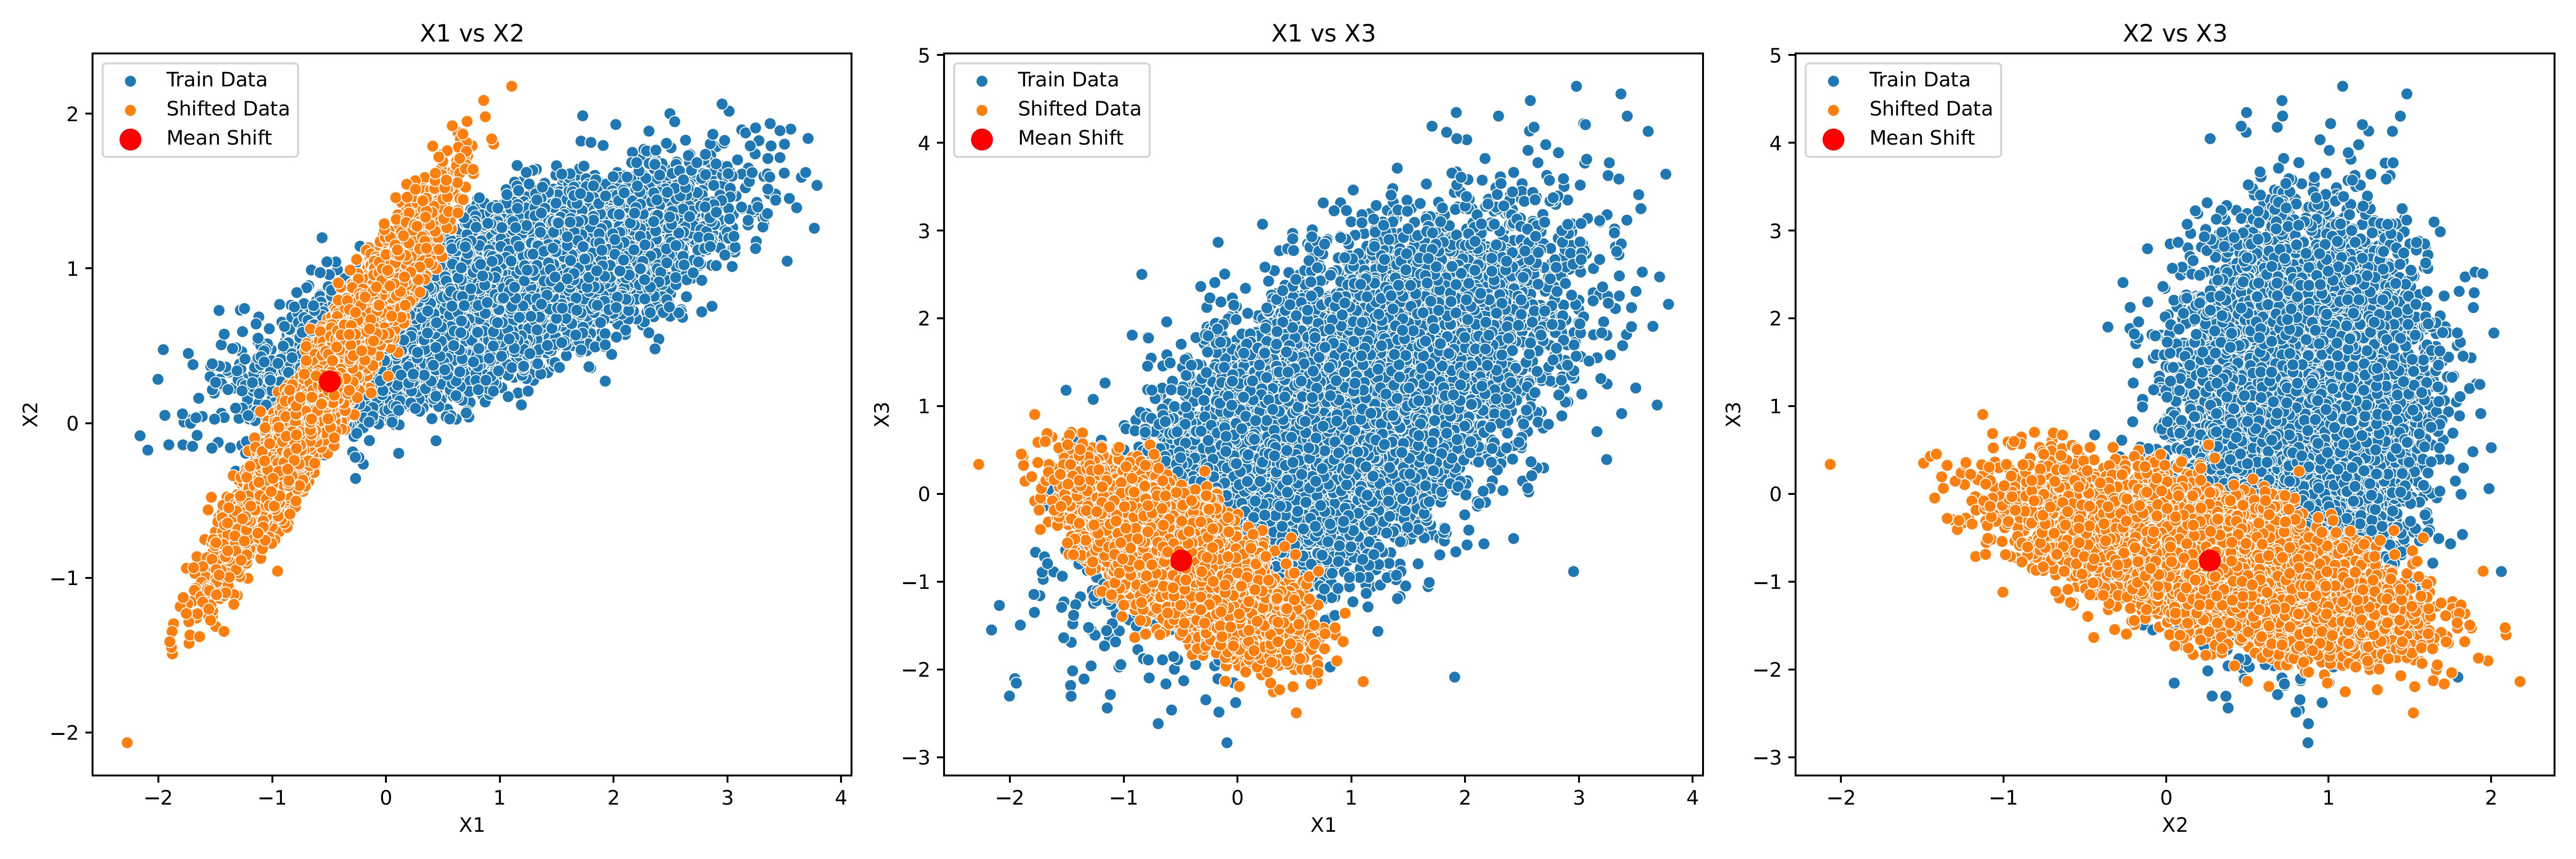
\includegraphics[width=\textwidth]{scatter_plots.jpg}
    \end{figure}
\end{frame}

\begin{frame}{Label Distribution in Train Set} 
    \vfill
    \centering
    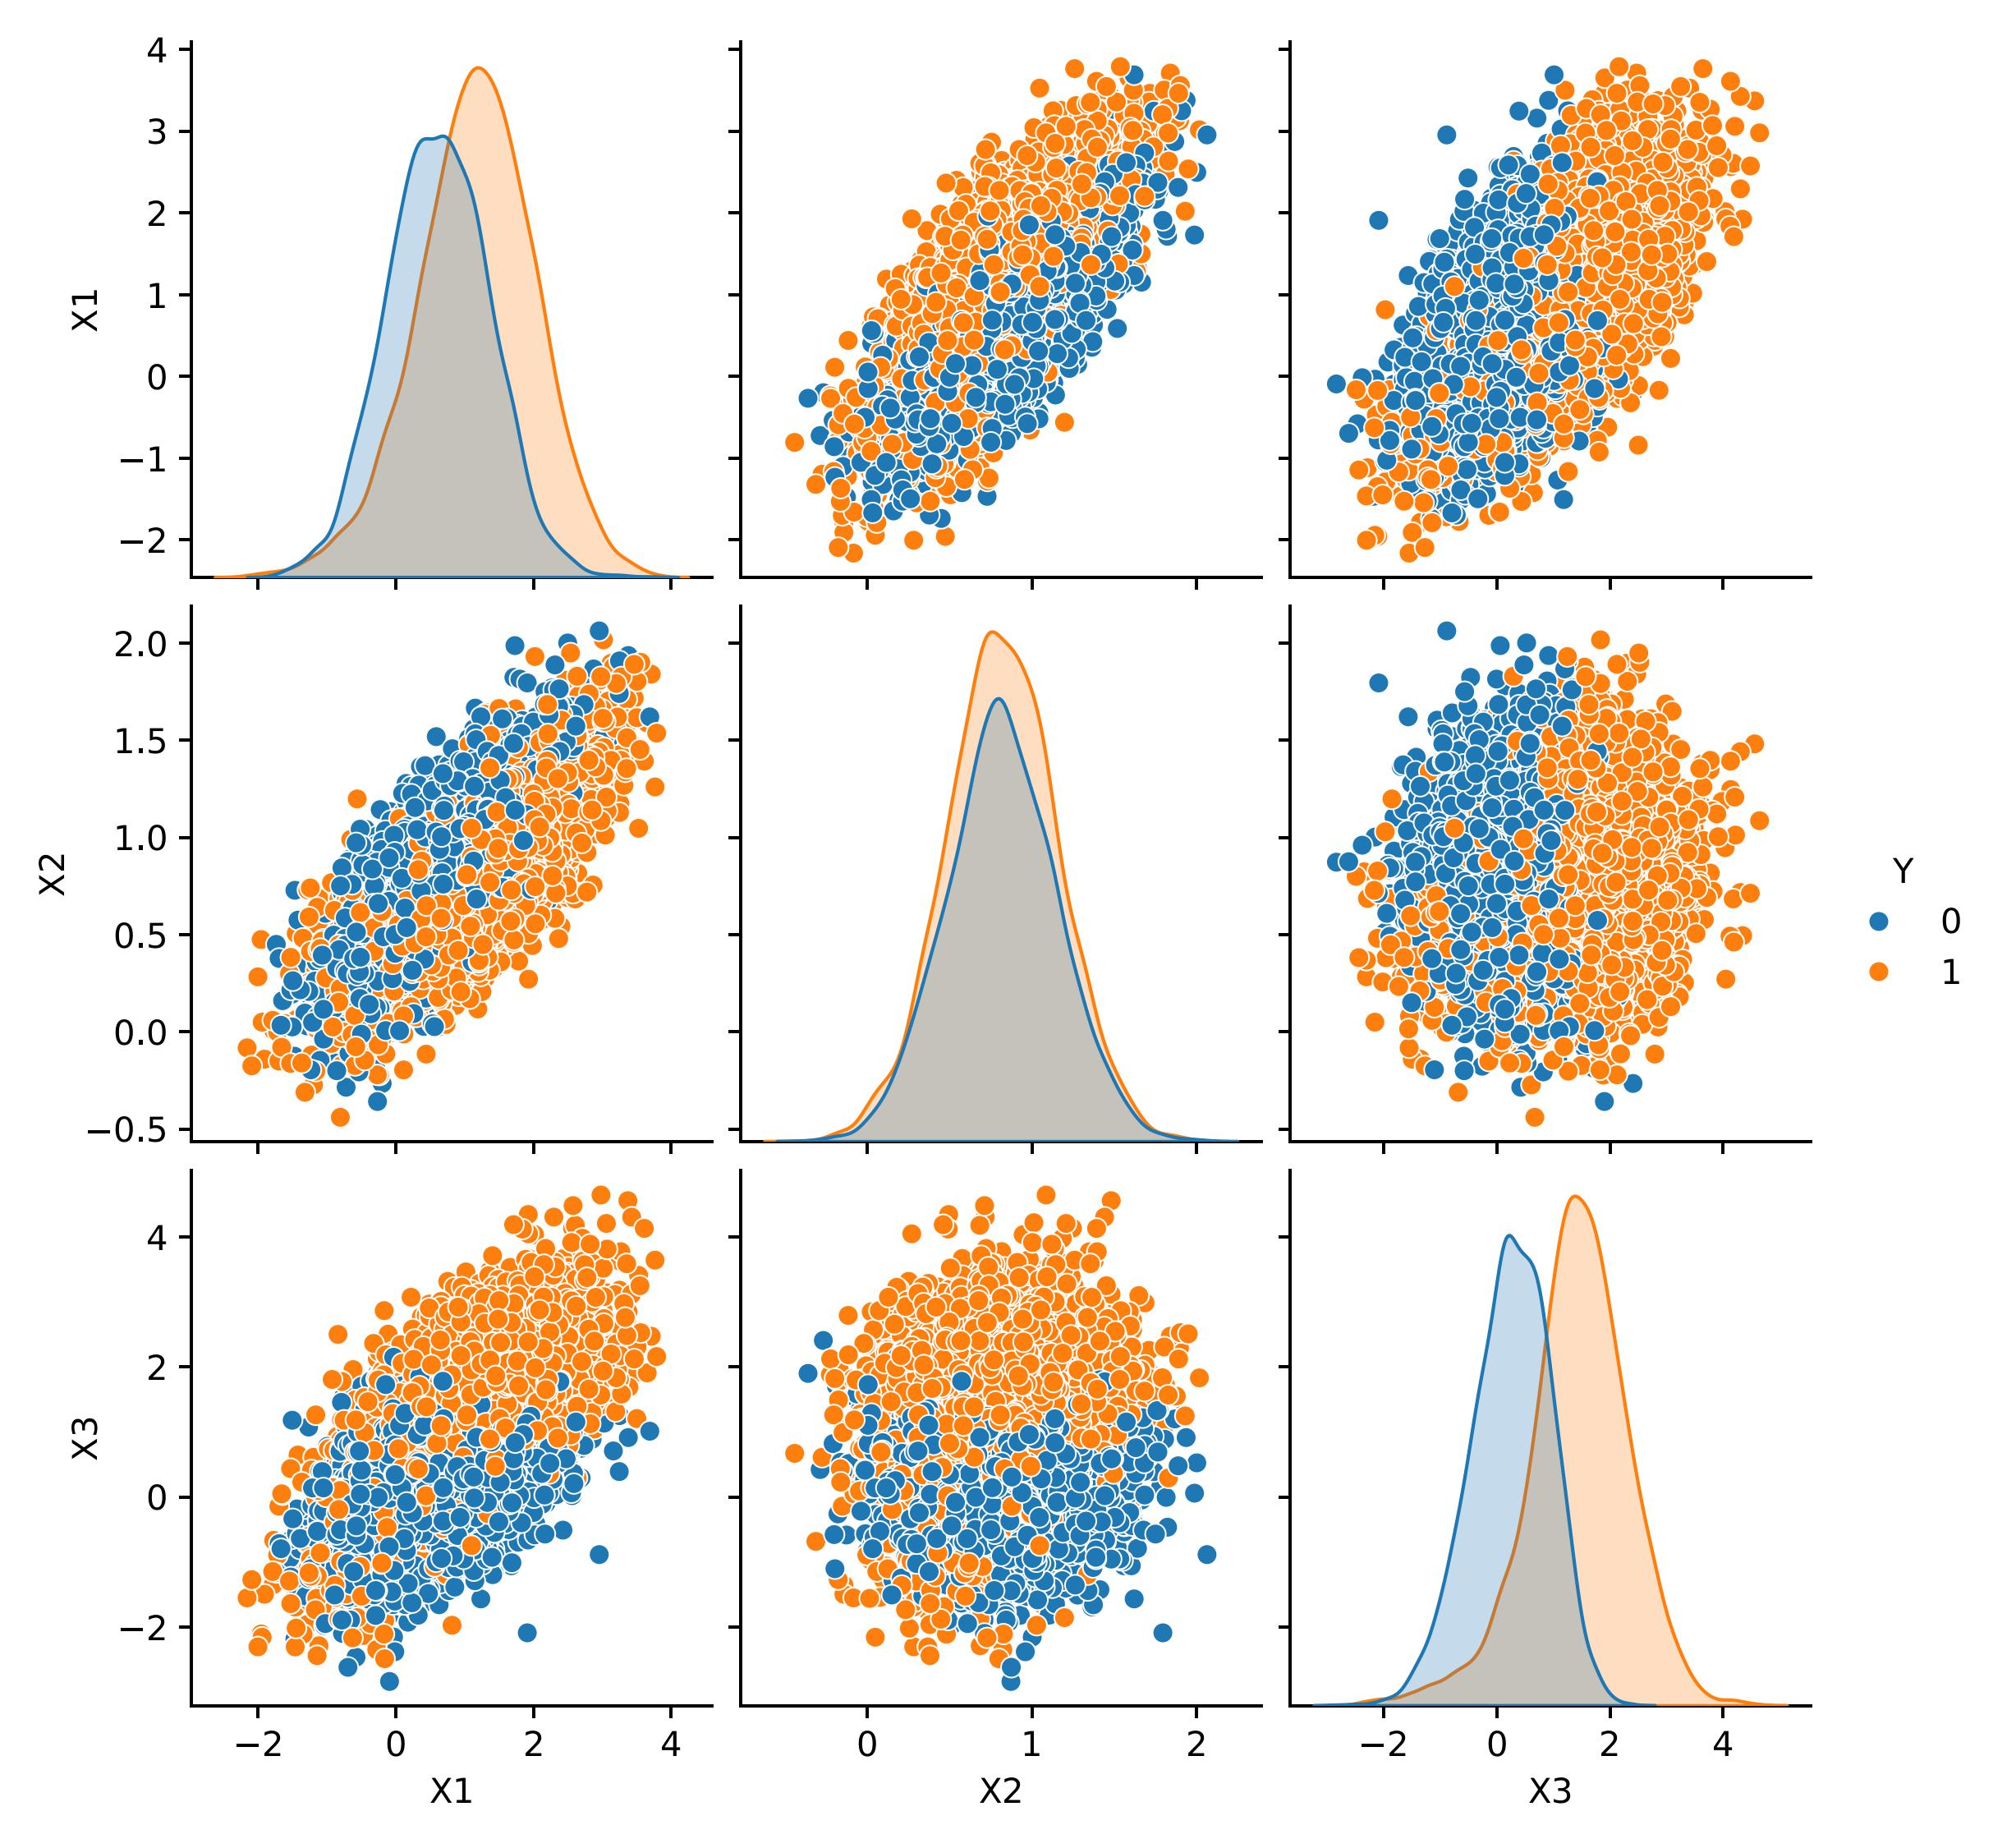
\includegraphics[width=0.7\textwidth]{pairplot.jpg}
    \vfill

\end{frame}

\begin{frame}{Label Distribution in Shifted Test Set}
    \begin{figure}
        \centering
        \vfill
        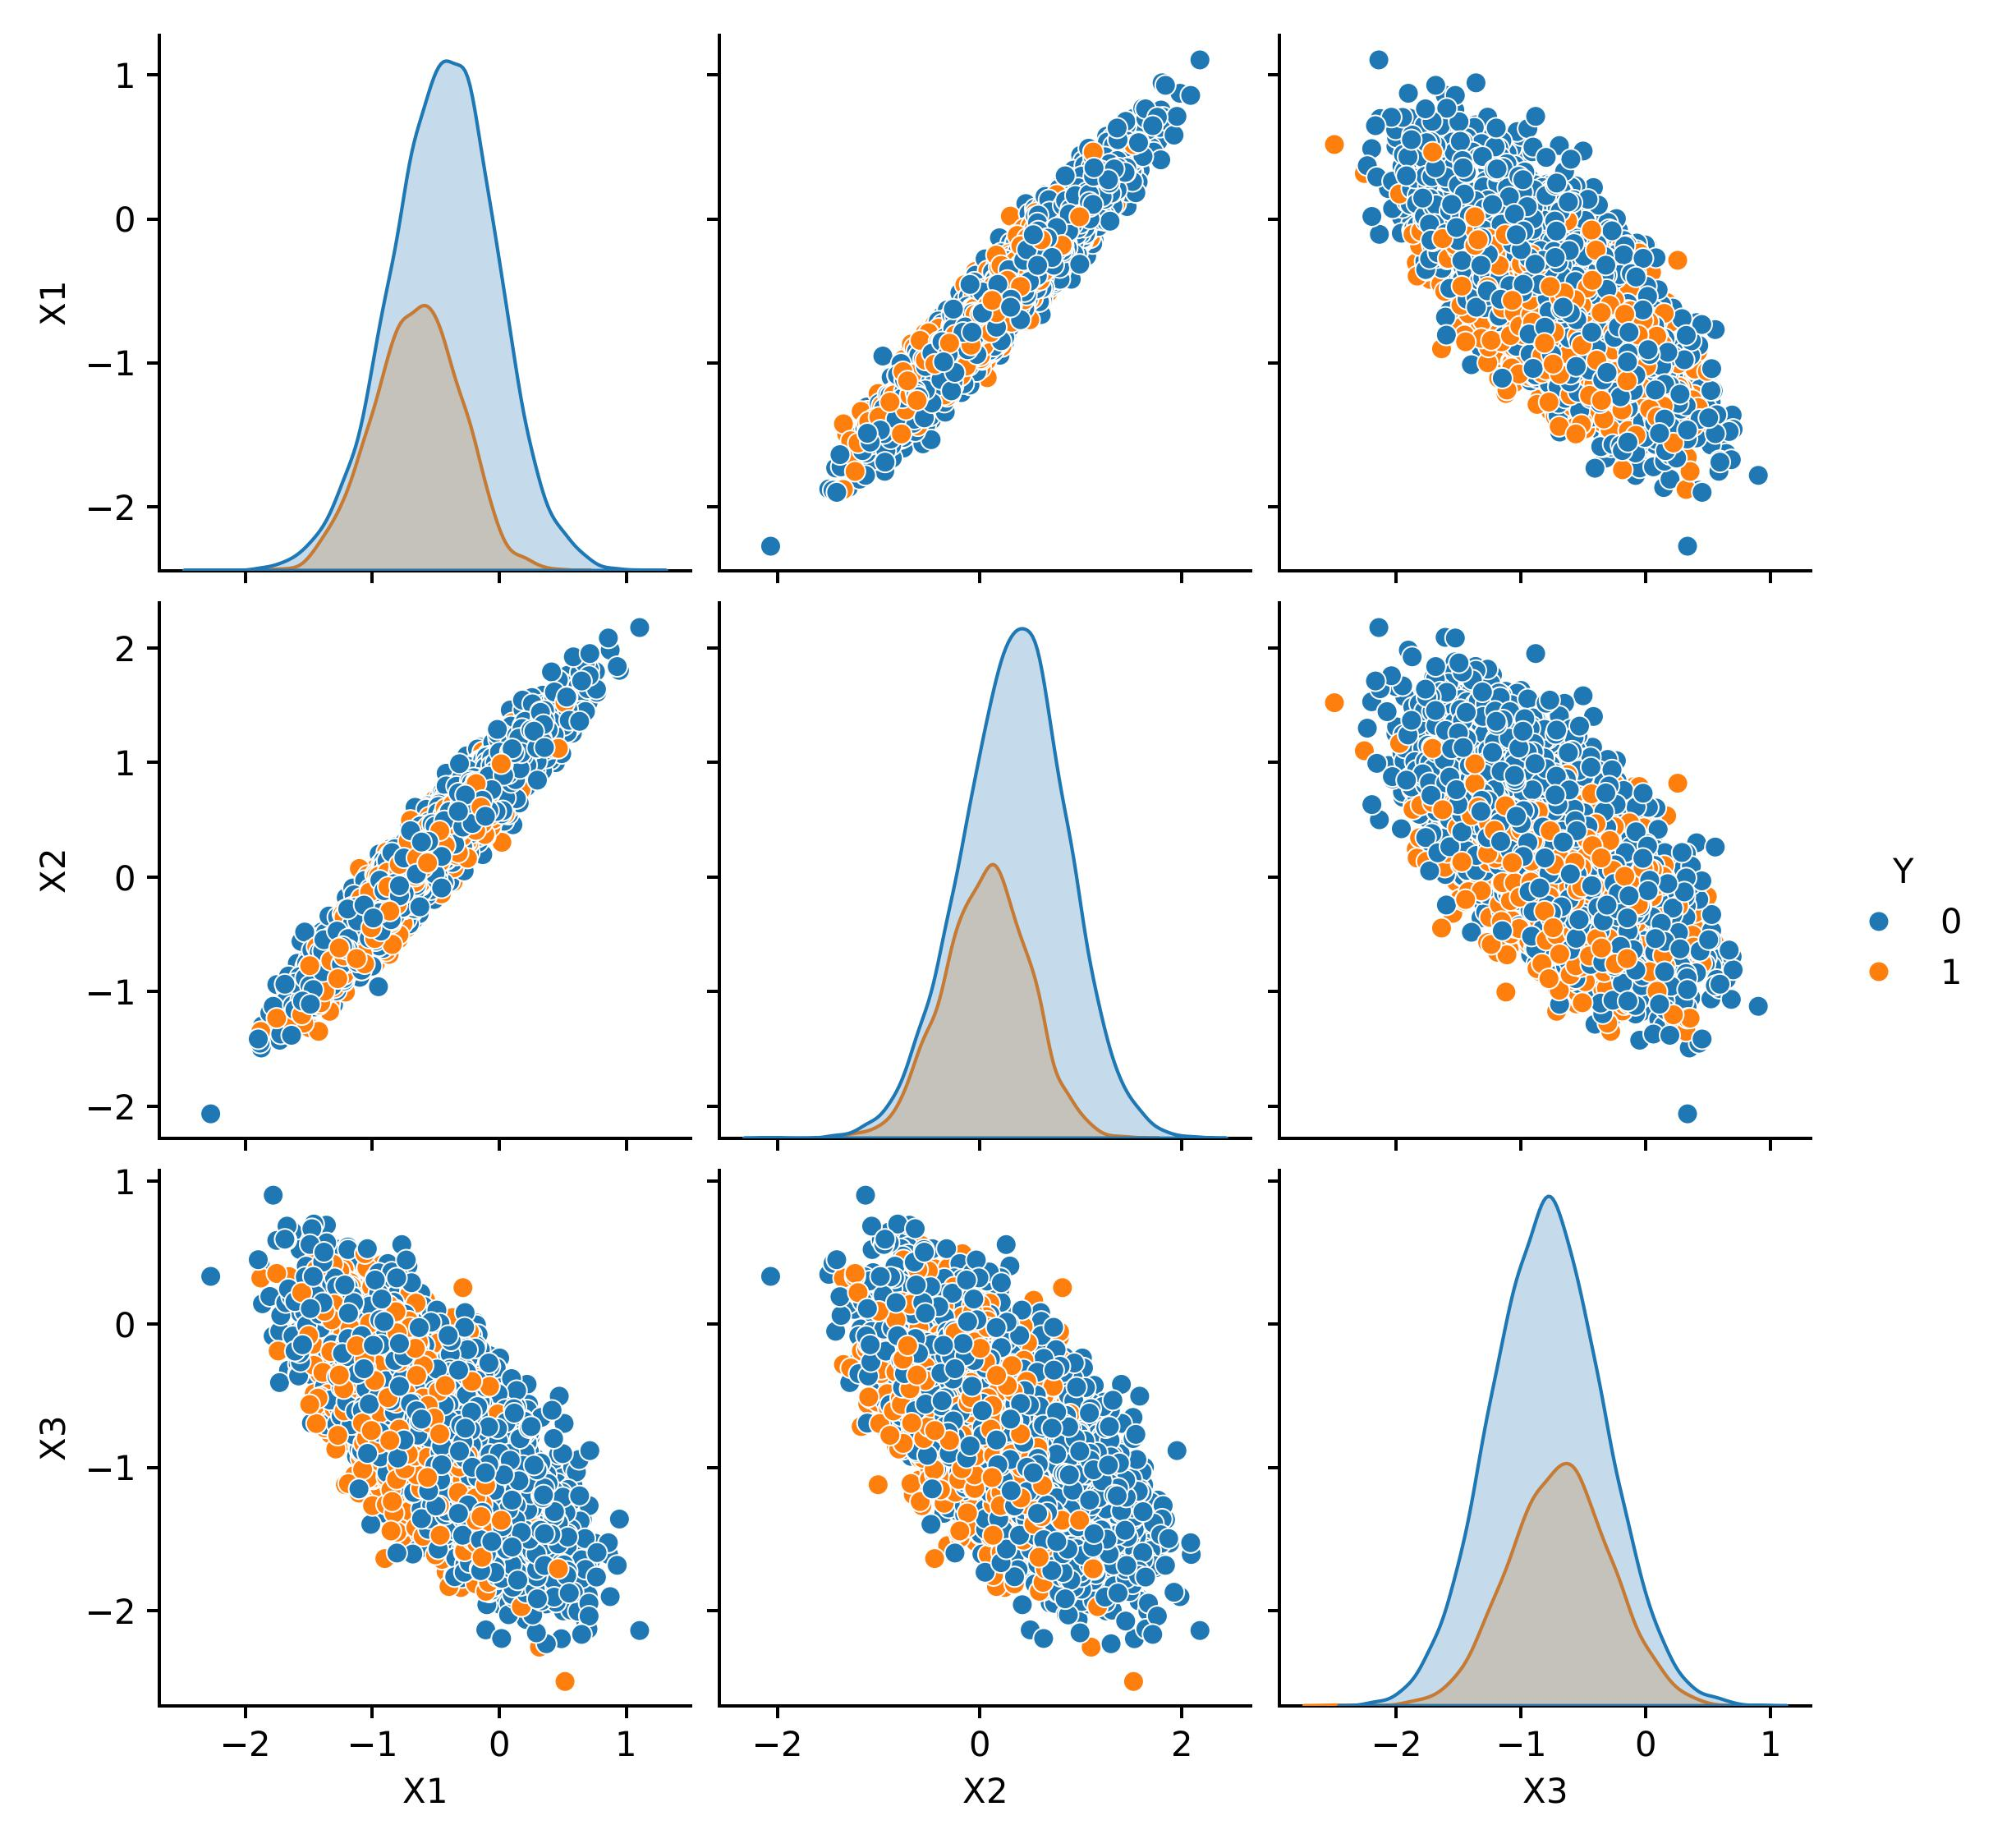
\includegraphics[width=0.7\textwidth]{pairplotshift.jpg}
    \end{figure}
\end{frame}

\begin{frame}{Testing Mixture}
    
    Series of datasets using \textbf{statistical mixtures} of the training features distribution and the fully shifted distribution.

    $$
    \boldsymbol{X}_\alpha \sim \alpha\cdot\mathcal{N}(\boldsymbol{\mu}_{\text{shift}}, \boldsymbol{\Sigma}_{\text{shift}}) + (1-\alpha)\cdot\mathcal{N}(\boldsymbol{\mu}_{\text{train}}, \boldsymbol{\Sigma}_{\text{train}})
    $$
    $$
    \alpha \in \{0.0, 0.1, \dots, 1.0\}
    $$
    $$
    Y_\alpha \text{ generated as before}
    $$

    \textbf{\underline{Note}:} $\boldsymbol{X}_{0.0}$ and $\boldsymbol{X}_{\text{train}}$ come from the same distribution, but the former are used as fresh new data.

\end{frame}

\begin{frame}
    \vfill
    \begin{figure}
        \centering
        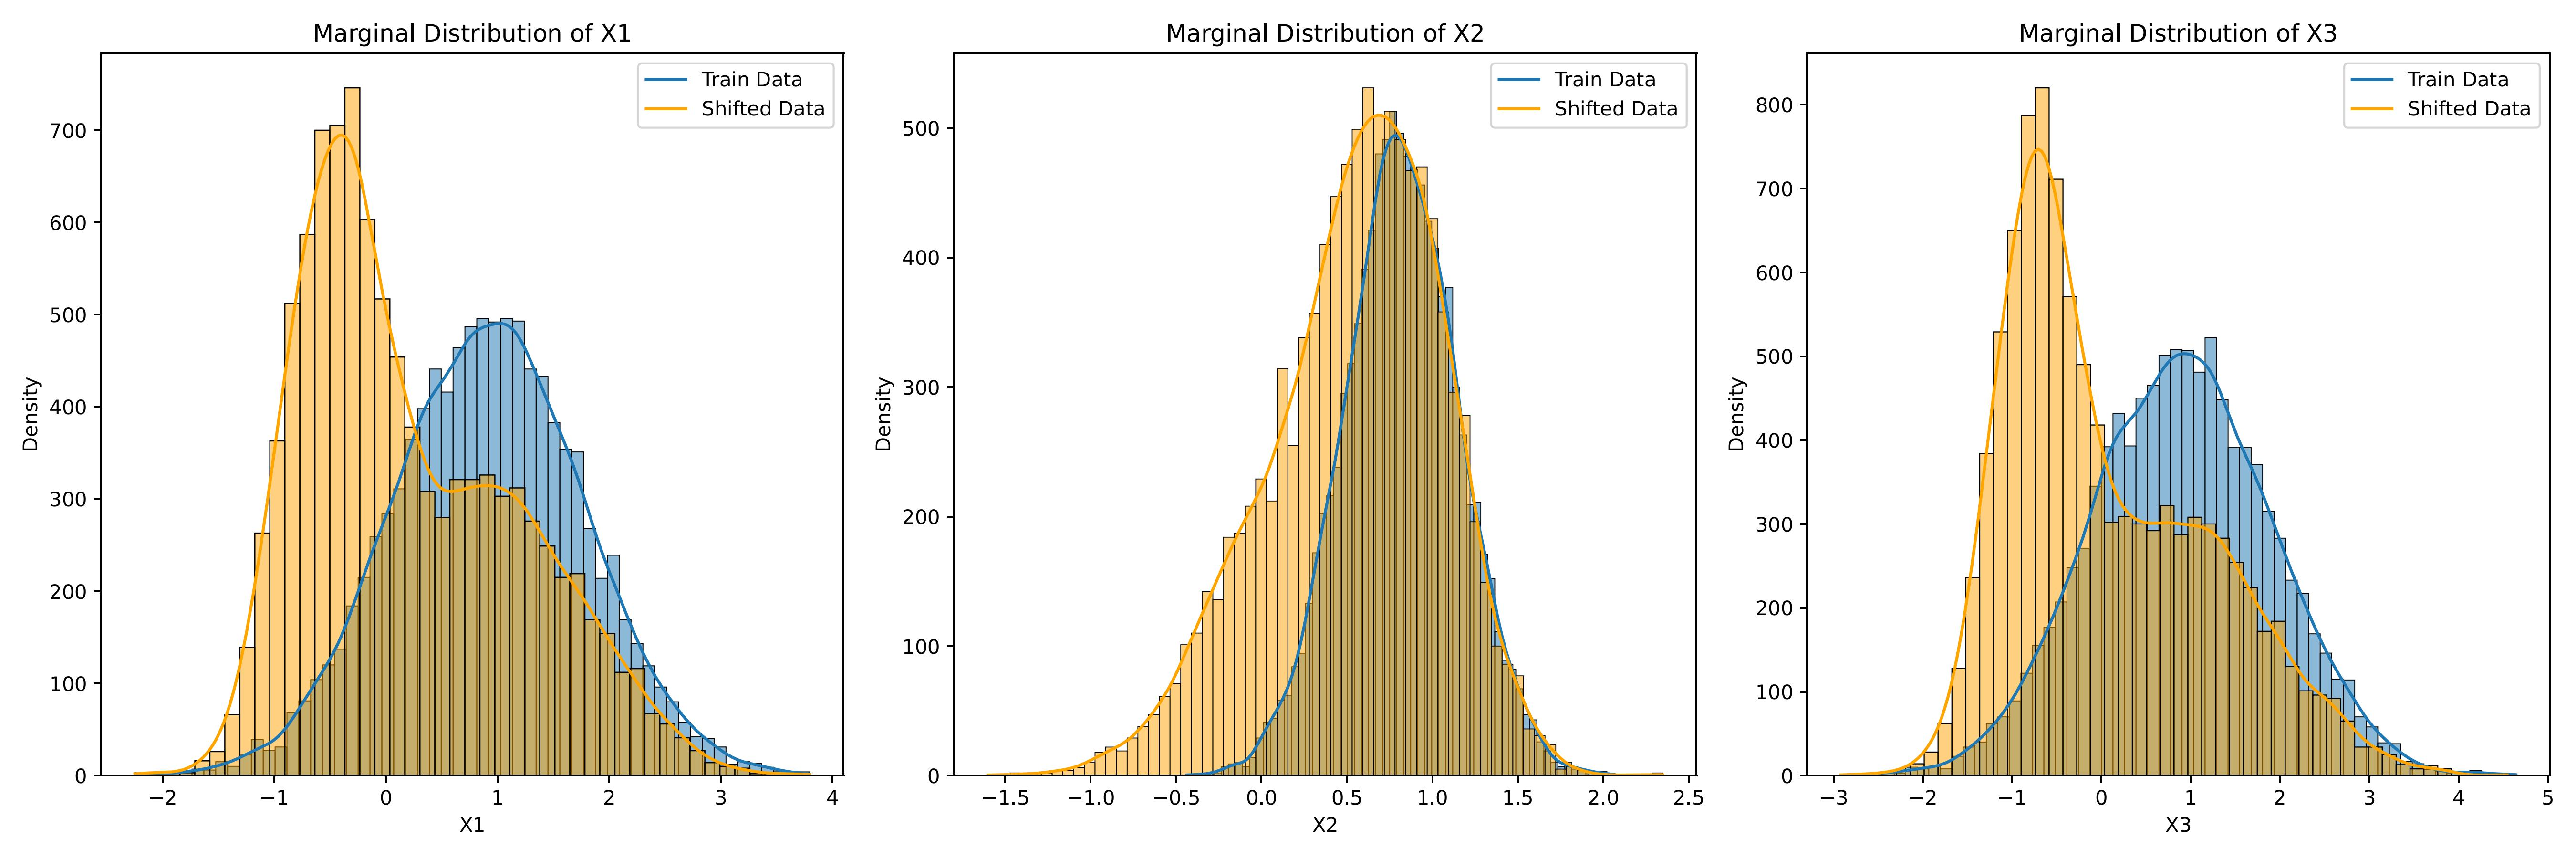
\includegraphics[width=0.9\textwidth]{marginal_plots0.5.jpg}
        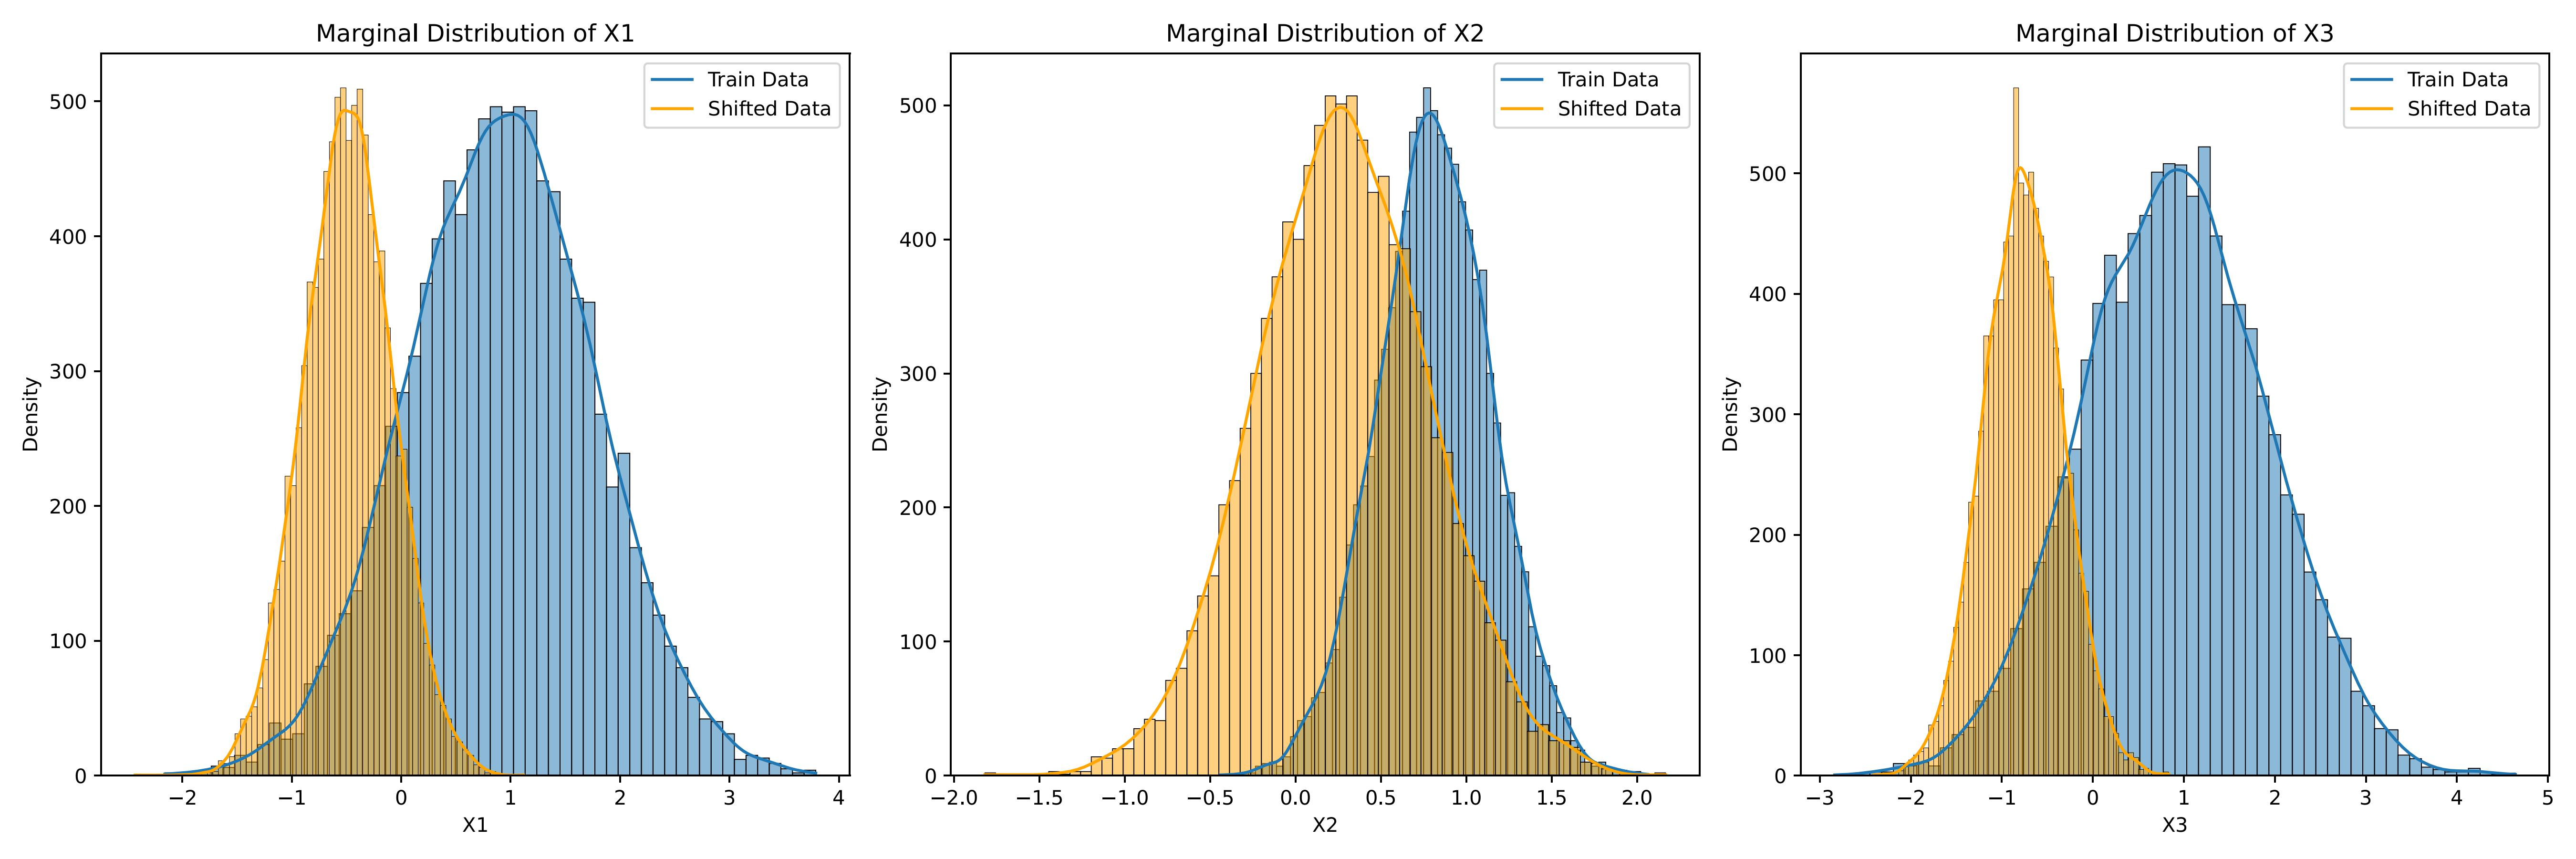
\includegraphics[width=0.9\textwidth]{marginal_plots1.0.jpg}
    \end{figure}
    Top: $\alpha=0.5$. Bottom: $\alpha=1.0$.
\end{frame}

